\subsection{Supervised Fine Tuning}
\label{subsec:SFT}
For \ourmodel SFT, we focused on improving dataset quality and diversity. In particular, we scaled up our agentic datasets and increased their share in the overall SFT blend. The chat template remains identical to \nanomodel. In addition, we add low effort reasoning mode, giving users further control over reasoning length. We found that a single-stage SFT led to a marked degradation on long-input-short-output scenarios. We therefore adopt a two-stage SFT procedure: Stage~1 emphasizes learning from token-level supervision and induces strong reasoning behavior, while Stage~2 switches to per-conversation normalization to prevent long outputs from dominating the loss, which restores long-input-short-output performance while retaining reasoning. We describe it below:

\subsubsection*{SFT objective and two-stage loss}

% We supervise the model only on \emph{output} (assistant) tokens, masking prompt tokens.
For a packed global batch $\mathcal{B}$ containing multiple conversations $c$, let $\mathcal{O}_c$ denote the set of output-token positions for conversation $c$ and $|\mathcal{O}_c|$ its output-token count. With token-level negative log-likelihood $\ell_t = -\log p_\theta(y_t \mid x, y_{<t})$, we use:

\paragraph{Stage 1: token-level (global) average.}
We minimize the average loss over \emph{all} output tokens in the packed global batch:
\begin{equation}
\mathcal{L}_{\text{tok}}
= \frac{\sum\limits_{c \in \mathcal{B}} \sum\limits_{t \in \mathcal{O}_c} \ell_t}
{\sum\limits_{c \in \mathcal{B}} |\mathcal{O}_c|}.
\end{equation}
This corresponds to summing the output-token log probabilities across all conversations and normalizing by the total number of output tokens.


\paragraph{Stage 2: sample-level average.}
We then switch to a per-conversation normalized loss and average equally across conversations:
\begin{equation}
\mathcal{L}_{\text{samp}}
= \frac{1}{|\mathcal{B}|} \sum\limits_{c \in \mathcal{B}}
\left(
\frac{1}{|\mathcal{O}_c|} \sum\limits_{t \in \mathcal{O}_c} \ell_t
\right).
\end{equation}
This stage reduces the dominance of long outputs by normalizing each conversation by its own output-token count before averaging across the batch.

For Stage 1, we run SFT with 256k sequence length packing, global batch size 64, constant lr $1e-5$ with 30k warmup samples.
 For Stage 2, we use 512k sequence length packing and include long context data with length up to 512K, global batch size 32 and constant lr $1e-5$. 

\paragraph{MTP during SFT} We continue training \ourmodel with the same shared-weight MTP head used in pretraining to preserve both the accuracy benefits of multi-step prediction and the inference-time gains from speculative decoding. Concretely, we train two MTP layers with shared parameters and optimize the combined objective using a scaled auxiliary loss computed with per-token loss and 0.3 scaling factor. 


\subsubsection{Data}

We reuse the following datasets from the \nanomodel SFT datasets: Chat, Infinibyte,  and Formal Proofs. We refresh the following datasets with new teacher models (\texttt{DeepSeek v3.2, Kimi K2}): Competition Math, Competition Code,  Conversational Tool Use, Multilingual, Science. Below we describe new or heavily modified SFT datasets.

\textbf{Software Engineering.}
We curate a dataset of coding tasks derived from real-world GitHub issues to train \ourmodel for autonomous software engineering capabilities including code exploration, task tracking, issue reproduction and bug fixing. We use the issues and containerized execution environments from the SWE-Gym \citep{pan2025trainingsoftwareengineeringagents}, R2E-Gym \citep{jain2025r2egymproceduralenvironmentshybrid} and SWE-rebench \citep{badertdinov2025swerebenchautomatedpipelinetask} datasets. For R2E-Gym, we regenerate problem statements with \texttt{Qwen3-Coder-480B-A35B-Instruct}. We distill trajectories from the OpenHands agent harness using \texttt{Qwen3-Coder-480B-A35B-Instruct} as the teacher model.

\textbf{Agentic Programming.}

\begin{figure}[t!]
    \centering
    % \includegraphics[width=\textwidth]{figures/agentic_pipeline.png}
    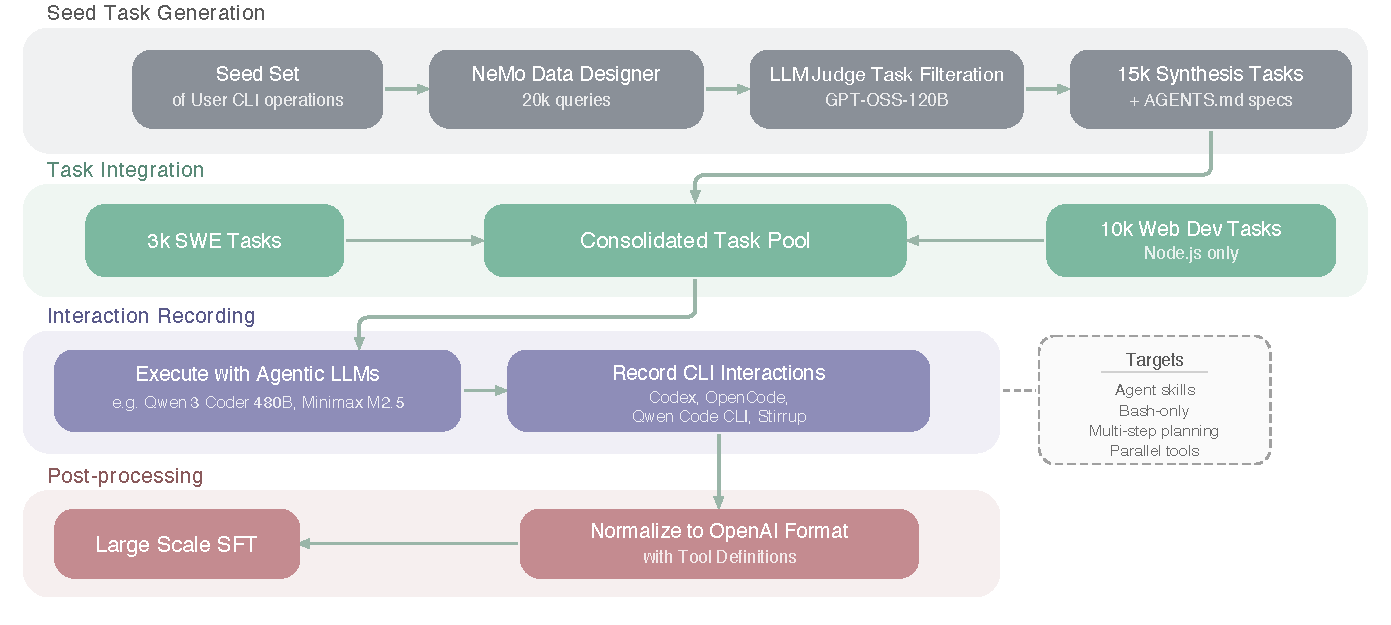
\includegraphics[width=\textwidth]{figures/swe-sft-data.pdf}
    \vspace{-1em} % Adjust spacing between image and text
    \caption{Agentic Command Line Interface Dataset Construction \& Training Pipeline}
    \label{figure:agentic_data_pipeline}
\end{figure}
% 
The landscape of software development has undergone a substantial shift with the emergence of Agentic Command Line Interface (CLI) tools, moving beyond the "autocomplete" era of 2021–2023 into a regime of autonomous execution. Alongside substantial improvements in harnesses such as Claude Code, OpenCode, and OpenAI’s Codex, models are now capable of operating as active digital collaborators, capable of multi-step reasoning, long-horizon execution, and end-to-end task orchestration. 

We established a foundational seed set of tasks designed to replicate common user-initiated operations within agentic CLIs. Refer to Figure \ref{figure:agentic_data_pipeline} where we discuss the full pipeline. We utilized NeMo Data Designer \citep{nemo-data-designer} to generate approximately 20k queries derived from a taxonomy of 24 distinct actions typically performed in these environments. Subsequently, we employed \texttt{GPT-OSS 120B} \citep{openai2025gptoss120bgptoss20bmodel} in an LLM-as-a-Judge framework to filter out tasks referencing pre-existing codebases or modifications to extant files. This mitigation ensures that the models do not attempt modification operations within empty directories—a scenario that frequently results in redundant and exhausted tool invocations during failed execution cycles. The resulting dataset comprises roughly 15k tasks centered on direct solution synthesis. To further enhance the diversity of the generated outputs, we coupled each task with a supplementary markdown specification, equivalent to an AGENTS.md file. These documents impose additional constraints and architectural requirements, effectively narrowing the design space and necessitating more complex, varied solutions from the agent.

Since we eliminate all tasks that require a pre-existing codebases, we augment this task set with roughly 3000 questions from SWE tasks that are challenging and come with pre-existing repository and specific git hash commit. We apply a simple prompt prior to the existing issue statements, stating that the execution environment does not have the library installed and therefore execution of unit tests should be avoided. This is a conscientious decision made to substantially reduce the engineering effort required to support per sample container based execution of each SWE task, reduce the number of tool calls and avoid large tool outputs due to multiple rounds of unit test executions. This further relaxes the constraints imposed on the agent to solve the issue, as there is no SWE specific prompt to guide the agent in solving the task. Finally, we synthesize 10k web development tasks using a taxonomy of 100 fine-grained tasks that are commonly requested by users as the seed, on which we apply LLM-as-a-Judge to eliminate tasks that require a pre-existing repository. We impose no restrictions on these tasks, but provide only a Node.js environment and expect the agent to setup and install all dependencies and plugins on its own.

Applying these task sets, we distill from high-performance, open-source agentic LLMs such as \texttt{Qwen-3-Coder-480B} \citep{qwen2025qwen25technicalreport} and \texttt{Minimax M2.5} \citep{minimax2025m2} by recording their interactions with various CLI environments, such as Codex, OpenCode, Qwen Code CLI, and Stirrup. These interaction traces are subsequently filtered, normalized into the standard OpenAI message format with various tool definitions, and utilized for large-scale SFT to effectively embed agentic operational knowledge within the model. For each Agentic CLI, we study the individual capabilities that exist and are commonly utilized. We apply the same task sets to target different capabilities, such as Agent Skills, tool restriction (bash only execution), ask user clarifying questions, single and multi step planning, static and dynamic multi turn conversations and parallel tool calling, depending on whether the specific CLI can accommodate these capabilities. 

\textbf{Long Context.}
We extend the long-context SFT dataset from \nanomodel with a more comprehensive synthetic data pipeline. To improve long-context multi-document reasoning, we construct a synthetic SFT dataset using long sequences from our pre-training blend, which contains books, papers, financial reports, code repositories, etc. We first cluster these documents by topic/domain and concatenate related documents to reach target sequence lengths, such as 128K, 256K, or 512K tokens. 
% Optionally, we use shorter excerpts (e.g., 128K if the target sequence length is 512K) during synthetic data generation while retaining the full concatenated context during SFT. 
For each long-context sample, we use an LLM to generate one or more QA pairs. The prompt requires questions to involve cross-document or cross-section navigation, ensuring information is scattered rather than localized. It strictly enforces multi-hop reasoning, requiring at least 4 to 7 distinct retrieval or reasoning steps. These steps mandate computational or logical processing, preventing simple copy-pasting, and often include explicit formatting instructions. Next, we generate 8 independent reasoning traces for each context-question pair. We apply semantic majority voting to group the answers, either by exact match or via an LLM judge. From the resulting majority group, we select the answer containing the shortest reasoning trace. 
% Finally, to ensure the dataset provides a meaningful learning signal, we apply difficulty filtering by having the target model evaluate the samples. Any instances that the target model can already answer correctly prior to fine-tuning are discarded. Throughout this pipeline, we utilize \texttt{Qwen3-235B-A22B-Thinking-2507} \citep{yang2025qwen3technicalreport} for QA generation, reasoning trace generation, and semantic majority voting. For the final difficulty filtering step, we employ \texttt{Qwen3-235B-A22B-Instruct-2507} \citep{yang2025qwen3technicalreport} as the judge. 
Additionally, we generate seven synthetic reasoning tasks to improve the model's ability to process context in a sequential, left-to-right manner. Specifically, synthetic snippets (generated using \texttt{Qwen3-235B-A22B-Thinking-2507}) are concatenated together to form long input context. The thinking traces are constructed by chaining rule-based reasoning steps, each of which includes relevant excerpts from the input context and tracking metadata, such as the frequency of query-related snippets.
%We also construct input context upto required length by concatenating records from ~\cite{nvidia/Nemotron-Personas-USA} and prepare questions emphasizing multi-hop reasoning and information aggregation. Context, question and answers are formatted via pre-defined templates and ground truth is derived by running sql queries on records.
We also construct long-context samples by concatenating records from~\citep{nvidia/Nemotron-Personas-USA} to reach the required sequence length. Questions are designed to emphasize multi-hop reasoning and information aggregation across records. Context, question, and answer are formatted using pre-defined templates, with ground-truth answers derived by executing SQL queries over the underlying records.

\textbf{Financial Reasoning.}
To construct a large-scale training corpus for financial reasoning, we employ a template-based synthetic data generation (SDG) pipeline that scales a curated seed set into hundreds of thousands of grounded question--answer pairs. The pipeline sources 565 expert-authored seed questions from the SecQue benchmark~\citep{benyoash2025secque}, a dataset of financial analysis questions anchored to SEC 10-K and 10-Q filings. These seeds are expanded combinatorially across S\&P~500 companies\footnote{\url{https://en.wikipedia.org/wiki/List_of_S\%26P_500_companies}, accessed 2025.} and fiscal years (2019--2024), where comparative questions are restricted to company pairs within the same GICS Sub-Industry to preserve semantic coherence. GPT-OSS-120B paraphrases each template instantiation, producing up to three diverse reformulations per combination. The resulting questions are mapped to relevant SEC filing sections using the original SecQue metadata, and the corresponding documents are converted to markdown with a configurable token limit. For answer generation, we adopt the GenSelect strategy~\citep{toshniwal2025genselectgenerativeapproachbestofn}: five candidate answers are sampled per question using GPT-OSS-120B with distinct random seeds, and a larger judge model (Qwen3-235B-A22B) selects the best response based on numerical accuracy, financial methodology, and logical soundness. A smaller model (Qwen3-30B-A3B) then classifies each pair as \texttt{ANSWERABLE} or \texttt{UNANSWERABLE}, retaining only those containing a complete, substantive response. Prior to supervised fine-tuning, the SDG output undergoes percentile-based outlier removal and deduplication. The resulting dataset comprises 366,243 financial Q\&A pairs with reasoning traces.

\textbf{CUDA.}
A large-scale synthetic CUDA dataset comprising 100K samples for kernel generation, repair, and optimization was constructed using a synthetic data generation pipeline based on \texttt{DeepSeek-R1} and \texttt{GPT-OSS-120B}. Seed questions were sourced from popular open-source libraries, NVIDIA library API surfaces, and BackendBench \citep{saroufim2025backendbench}. These seeds were used to generate tuples of the form (PyTorch reference, CUDA C++ kernel) and (natural language specification, CUDA C++ kernel), each accompanied by reasoning. For each seed item, multiple candidate kernels were generated and rigorously validated for correctness within an internal CUDA evaluation environment. The validated kernels were then ranked by performance, and the highest-performing kernel was retained. In addition, we collected traces from an internal CUDA agent, producing samples of the form (PyTorch reference, faulty CUDA C++ kernel, error message, corrected CUDA C++ kernel) and (PyTorch reference, slow CUDA C++ kernel, Nsight Compute log, optimized CUDA C++ kernel). Using publicly available documentation and official code samples, and following the same formulation as the CUDA-C data, we generated additional PyTorch references and corresponding CUDA-library implementations with reasoning chains, as well as aligned natural language specifications. These libraries include Thrust, CUB, cuBLAS, cuDNN, cuSPARSE, cuRAND, and cuSOLVER.

% NOTE, Prasoon: I shortened it even further from our already shortened version, but we've something brand new in the SDG generation method so need some space to explain., @soumye/@alex if you feel there is need to still shorten more, please reach out to me/Makesh again.
\textbf{Safety.} We have significantly enhanced our safety framework compared to \nanomodel by combining a robust prompt library with a two-stage synthetic response generation strategy. While retaining the core prompts from Nemotron Content Safety v2 \citep{ghosh-etal-2025-aegis2}, Gretel Safety Alignment v1 \citep{gretelai_gretel-safety-alignment-en-v1}, Harmful Tasks \citep{hasan2024pruning} and Red-Team-2K \citep{luo2024jailbreakv_robustness} covering content safety and common jailbreak techniques, we added in new synthetic prompts targeting the elicitation of over-refusals, demographic biases, and copyright reproduction. We also expand coverage of jailbreak strategies to better capture emerging adversarial techniques including indirect prompt injection attacks. 

Our primary advancement over \nanomodel is an explicit response policy framework. For each prompt, a response policy is inferred from a combination of prompt metadata, its annotated safety category, and predictions from a set of lightweight auxiliary classifiers that detect attributes such as self-harm risk, demographic targeting, or the presence of embedded adversarial instructions. We cast this decision process as a multi-class classification problem, where each class corresponds to a distinct response mode aligned with safety guidelines. These response modes specify whether the model should provide supportive resources such as helpline information, issue a refusal with a brief explanation, or answer the benign portion of the request while ignoring malicious content. This ensures that the responses are safe, contextually appropriate, and consistent across a diverse set of safety-sensitive scenarios.

Following the deliberative alignment framework \citep{guan2025deliberativealignmentreasoningenables}, we adopt a two-stage generation process in which the reasoning trace and the final response are curated separately but consistently with our response policy. In the first stage, we construct a concise reasoning trace that guides the model to reflect on the safety properties of the prompt, explicitly identifying why the request may be unsafe or policy-relevant and what constraints should govern the response. In the second stage, we generate the final response based on this reasoning trace, ensuring that it adheres to the predefined response policy and behavior guidelines. This structured separation encourages deliberate reflection on safety guidelines while producing responses that are consistent, policy-compliant, and contextually appropriate to ensure that the final response follows safety policies while minimizing unnecessary references to said policies. Finally, we apply a content-moderation classifier to filter any responses flagged as unsafe, providing an additional safeguard to ensure alignment with safety objectives.

\textbf{Search.}
To improve search capabilities, we generated a synthetic search-agent SFT dataset using NeMo Data Designer \citep{nemo-data-designer}. The pipeline begins by constructing seed prompts grounded in the Wikidata knowledge graph \citep{vrandecic2014wikidata}: we query SPARQL \citep{sparql2013} for well-connected hub entities across approximately 25 verified entity classes (cities, universities, films, chemical elements, etc.), then perform random walks of 4-8 hops through the graph, filtering out degenerate paths via stop-node lists, anti-meta-relation exclusions, and minimum path-length thresholds. Each valid walk yields a start entity, a chain of factual relations, and a final answer entity.

Data Designer then processes these seeds in three stages: (1) a draft stage converts the structured knowledge-graph walk into a natural-language multi-hop question, (2) an obfuscation stage rewrites the question to hide intermediate entities and eliminate breadcrumb-style chaining -- producing search-riddle queries where the solver must decompose the problem independently -- and (3) an agent stage in which MiniMax-M2 \citep{minimax2025m2} solves the obfuscated question by issuing web searches via the Tavily (\url{https://tavily.com}) MCP search tool, producing a grounded search trajectory with supporting URLs. Each resulting SFT record is a multi-turn conversation where assistant turns interleave chain-of-thought reasoning with structured tool calls, and tool-response turns return search results as JSON, preserving a full Thought--Action--Observation loop across an average of 12 tool calls per trajectory. A final structured-output stage normalizes the agent's raw response into a validated JSON schema. 
% Pre-generation filters remove seeds with generic or abstract answer entities, and post-generation validators discard samples lacking tool calls, supporting URLs, or substantive justifications, yielding approximately 7K training records.


\textbf{Terminal Use.}
The dataset for enhancing terminal capabilities follows the dual-stream \textit{Terminal-Task-Gen} methodology described in Nemotron-Terminal \citep{pi2026dataengineeringscalingllm}, comprising a total of 84,864 samples. This pipeline combines the adaptation of existing high-quality datasets with synthetic task generation grounded in a comprehensive terminal skill taxonomy. The source distribution consists of 68,924 synthetic samples, 8,125 samples from Nemotron-Cascade-Math, and 7,815 samples from Nemotron-Cascade-Code \citep{wang2025nemotroncascadescalingcascadedreinforcement}. For trajectory construction, we use \texttt{DeepSeek-V3.2} \citep{deepseekai2024deepseekv32} as the primary engine to generate step-by-step solution traces within isolated, Dockerized environments through an agentic execution-feedback loop. All samples are generated using the Terminus 2 agent framework~\citep{merrill2026terminalbenchbenchmarkingagentshard} as the underlying scaffolding, providing a unified set of terminal tools and a structured interaction protocol to maintain consistency and quality across long-horizon trajectories.

\textbf{Multilingual.}
Our multilingual data combines synthetic translations of English SFT examples with a sentence-level parallel corpus to improve machine translation. We reuse the line-by-line translation pipeline from \nanomodel, translating into six languages (German, Spanish, French, Italian, Japanese, and Chinese) using \texttt{Qwen2.5-Instruct-14b}. After translation, we apply filtering to remove samples in the wrong language and other common failure modes. We observed a recurring pattern where translation disrupts the alignment between prompt specifications and answer formats — a consistency usually maintained in English data. This mismatch led to instruction-following failures during preliminary testing. To mitigate this, we introduced a lightweight post-editing step with \texttt{Qwen3-4B-Thinking-2507} to automatically restore format compliance. We also expand the parallel corpus with additional Chinese $\leftrightarrow$ English pairs and exclude very short samples that previously degraded post-training performance.


\textbf{Structured Query Language (SQL).}
To improve \ourmodel on enterprise SQL workloads, we generate a synthetic text-to-SQL dataset with NeMo Data Designer \citep{nemo-data-designer}. The dataset contains 96.5k records spanning MySQL, PostgreSQL, and SQLite across 60 industry sectors, $\sim$700 domain topics, and 90 SQL concept buckets (from basic SELECT to recursive CTEs, window functions, and geospatial queries). Each sample pairs a natural-language prompt and a fully synthetic database schema context with a target SQL query. To improve robustness and to mimic the real-world messiness of production databases, the pipeline injects distractor tables and columns into the database context. Specifically, related but irrelevant tables and columns are added to the database context, forcing the model to learn to ignore irrelevant schema elements. Prompt diversity is controlled along three axes -- instruction style (imperative, declarative, interrogative, contextual, abbreviated), linguistic register (formal, conversational, technical, academic, direct), and politeness level -- yielding naturalistic and varied user requests. The final dataset of 96.5k records is validated and filtered down by Data Designer from a larger dataset using per-dialect syntax validators and five LLM-as-a-critic judges.

% \textbf{Conversational Tool Use.} Creating a large set of broad and specialized tool-use data for training has been adopted into many models to boost agentic capabilities \citep{Liu2024ToolACE,deepseekai2024deepseekv32,kimiteam2025kimik2openagentic,5team2025glm45agenticreasoningcoding}. For \ourmodel, we scale the conversational tool use data by creating a fully synthetic, 6-stage data generation pipeline.
% \begin{enumerate}
%     \item Domain Generation: We sample multiple synthetic domains using a model, iteratively asking the model to build upon it's initial generation to further sample specialized subdomains.
%     \item Policy and Tool Generation: We use a model to sample various customer-service policies and related tools an agent can use, iteratively improving the sampled policies and tools using self-refinement. To maintain policy style and formatting, we use a few-shot prompt and utilize LM-as-a-Judge to filter for quality.
%     \item Scenario Generation: We use a model to generate a set of plausible user personas, background information, and inquiries for each policy setting.
%     \item Trajectory Collection: Using the policy and scenario pairs, we conduct $16$ customer service interactions between a model-simulated agent, user, and environment using the policy and scenario pairs.
%     \item Verification: We judge the quality of each trajectory in both the outcome and process level using LM-as-a-Judge.
%     \item SFT Data Selection: We choose successful trajectories for SFT training, filtering for difficulty by dropping all scenarios that resulted in all-success or all-failure.
% \end{enumerate}

\textbf{Conversational Tool Use.} Large-scale specialized tool-use training data has been adopted by many models to boost agentic capabilities \citep{Liu2024ToolACE,deepseekai2024deepseekv32,kimiteam2025kimik2openagentic,5team2025glm45agenticreasoningcoding}. For \ourmodel, we scale conversational tool-use data via a fully synthetic, six-stage generation pipeline:
\vspace{-0.25\baselineskip}
\begin{enumerate}
\item Domain Generation: Sample synthetic domains with a model, iteratively expanding initial generations into specialized subdomains.
\item Policy and Tool Generation: Sample customer-service policies and related tools, iteratively improving them via self-refinement; use few-shot prompting and an LM-as-a-Judge for quality filtering to maintain style and formatting.
\item Scenario Generation: Generate plausible user personas, background information, and inquiries for each policy setting.
\item Trajectory Collection: For each policy–scenario pair, simulate $16$ customer service interactions among a model-based agent, user, and environment.
\item Verification: Evaluate trajectories at both outcome and process levels using an LM-as-a-Judge.
\item SFT Data Selection: Select successful trajectories for SFT and filter for difficulty by dropping scenarios that yield all-success or all-failure outcomes.
\end{enumerate}

\begin{figure}[!t]
\centering
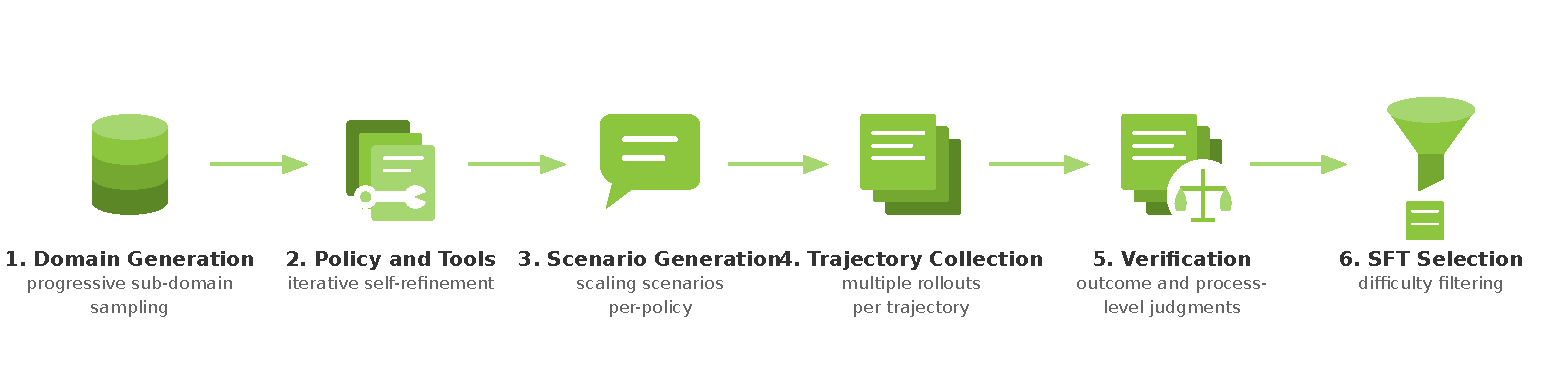
\includegraphics[width=0.9\linewidth]{figures/conversational_tool_use_data_generation.pdf}
\caption{Overview of the synthetic data generation pipeline for specialized conversational tool-use SFT data used for \ourmodel.}

\label{fig:conversational_tool_use_data_generation_pipeline}
\end{figure}


A visualization of the pipeline is shown in Figure \ref{fig:conversational_tool_use_data_generation_pipeline}. We utilize \texttt{Qwen3-235B-A22B-Thinking-2507}, \texttt{Qwen3-32B}, \texttt{Qwen3-235B-A22B-Instruct-2507} \citep{yang2025qwen3technicalreport}, \texttt{deepseek-r1-0528} \citep{deepseekai2025deepseekr1incentivizingreasoningcapability}, \texttt{DeepSeek-V3.2} \citep{deepseekai2024deepseekv32}, and \texttt{gpt-oss-120b} \citep{openai2025gptoss120bgptoss20bmodel} on various parts of the above pipeline, yielding 279{,}116 conversations across 838 domains. This represents a substantial scale-up over \nanomodel, which used 15{,}588 conversations spanning 5 domains.


\textbf{General-Purpose Tool Use.}
The broader, general purpose tool-calling synthetic data pipeline begins with the construction of diverse tool sets from ToolEyes \citep{ToolEyes2025}, API-Bank \citep{APIBank2023}, UltraTools \citep{Huang2024UltraTool}, AutoTools \citep{Shi2025AutoTools}, xLAM \citep{Zhang2024xLAM}, Glaive-Function-Calling-v2 \citep{GlaiveFunctionCallingV22025}, Toucan-1.5M \citep{Xu2025Toucan}, as well as custom written tools that serve as the foundation for downstream synthetic task generation. A tool-calling trajectory is simulated by grounding in one or multiple of these tool sets. The trajectory simulation involves an LLM playing three roles - User (User-LLM), Assistant (Assistant-LLM), and Tool Environment (Tool-LLM). The User-LLM is seeded with the selected tool set, a persona sampled from Nemotron-Personas-USA \citep{nvidia/Nemotron-Personas-USA}, and a tool-calling scenario (single-turn, multi-turn, or multi-step). The User-LLM starts by designing a task guided by the tool-calling scenario which is relevant to the selected persona and can be solved by the selected tool set. The Assistant-LLM attempts to solve this task in one or more turns by producing tool-calls and responding to tool execution results. The Tool-LLM is responsible for producing a simulated tool execution result based on the tool-call generated by the Assistant-LLM and the tool being called. The Tool-LLM is prompted with a rubric that helps identify syntactic and semantic errors in tool-calling, as well as the original user query so that the tool results can be contextualized when tool-call is successful. To ensure accuracy, we employ a turn-level and trajectory-level judge similar to the specialized tool-calling data generation. The turn level judge is also paired with a rule-based verification for ensuring correctness of tool-calls. We scale this pipeline with DeepSeek-v3.2 \citep{DeepSeekV32025} and GLM-4.7 \citep{GLM47Zai2025} to create a dataset of 1.5M diverse tool-calling trajectories.

The overall general-purpose synthetic tool-calling data pipeline is visualized in figure \ref{fig:broad_conversational_tool_use_data_generation_pipeline}.

\begin{figure}[!t]
\centering
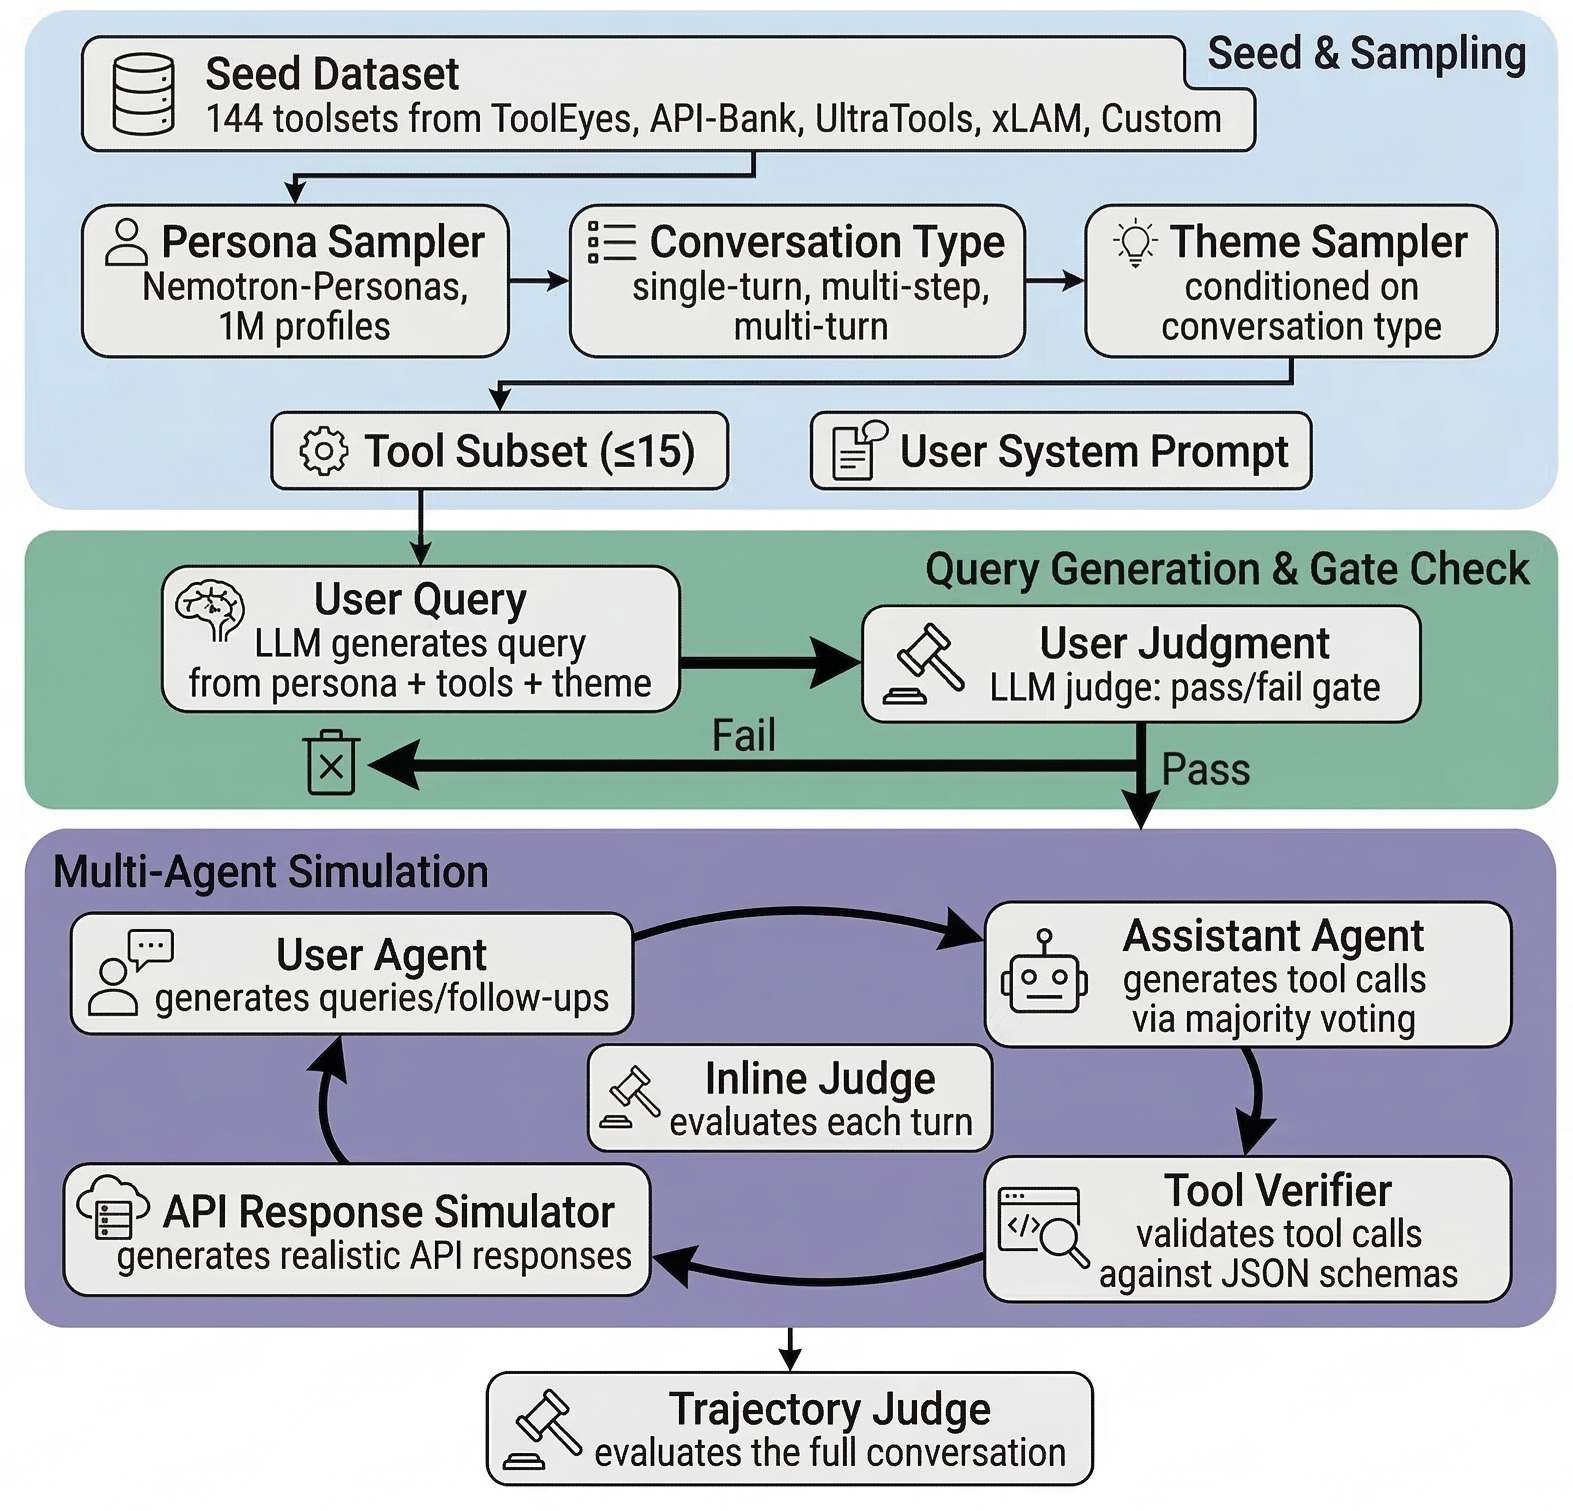
\includegraphics[width=0.5\linewidth]{figures/broad_conversational_tool_use-new.png}
% change the image to match template
\caption{Overview of the pipeline for general-purpose tool-calling data used in \ourmodel.}

\label{fig:broad_conversational_tool_use_data_generation_pipeline}
\end{figure}

% A comparison of the scale of SFT data used in model training compared to \texttt{\nanomodel} is shown in Table \ref{tab:conversational_tool_use_data_size}.
% \begin{table}[!t]
% \centering
% \begin{tabular}{lcc}
% \hline
% \textbf{Model} & \textbf{Number of Domains} & \textbf{Number of Conversations} \\ \hline
% \nanomodel & 5 & 15588 \\
% \ourmodel & 838 & 279116 \\ \hline
% \end{tabular}
% \caption{Size of conversational tool-use data used in SFT for \nanomodel vs \ourmodel. Using our synthetic data generation pipeline, we greatly increase the diversity and scale of the data by increasing the number of domains and conversations.}
% \label{tab:conversational_tool_use_data_size}
% \end{table}
% % 

% We generate synthetic multi-turn trajectories to demonstrate conversational tool use. The generation of these trajectories involves a user that is given a task to accomplish, an agent that is instructed to help the user accomplish their task, and a tool execution environment, each of which is simulated by a language model. To limit the trajectories in the SFT training data to ones in which the actions of all of these entities are consistent with their goals, we employ a language model as a judge to evaluate the trajectories, and filter out trajectories for which the judge considers an action of an entity to be inconsistent with its goals. We use Qwen3-235B-A22B-Thinking-2507 \citep{yang2025qwen3technicalreport}, Qwen3-32B \citep{yang2025qwen3technicalreport}, GPT-OSS-120b \citep{openai2025gptoss120bgptoss20bmodel}, and Qwen3-235B-A22B-Instruct-2507 \citep{yang2025qwen3technicalreport} to generate data in this synthetic tool use trajectory generation pipeline.

% \subsubsection{Data Filtering}
% We apply the same filtering process as Nemotron Nano v3.

\subsubsection{SFT Data Blend}
Our general stage 1 SFT data blend can be found in Figure \ref{fig:sft_blend} (all datasets not listed make up less than 1\% of the blend). We train on over 7M total samples. In stage 2, we use 85\% of the stage 1 blend and augments it with 256K and 512K-token long-context data. Compared to \nanomodel, we  significantly increased the volume and diversity of agentic tasks, and allocate it a much larger proportion of our blend.

\begin{figure}[t]
    \centering
    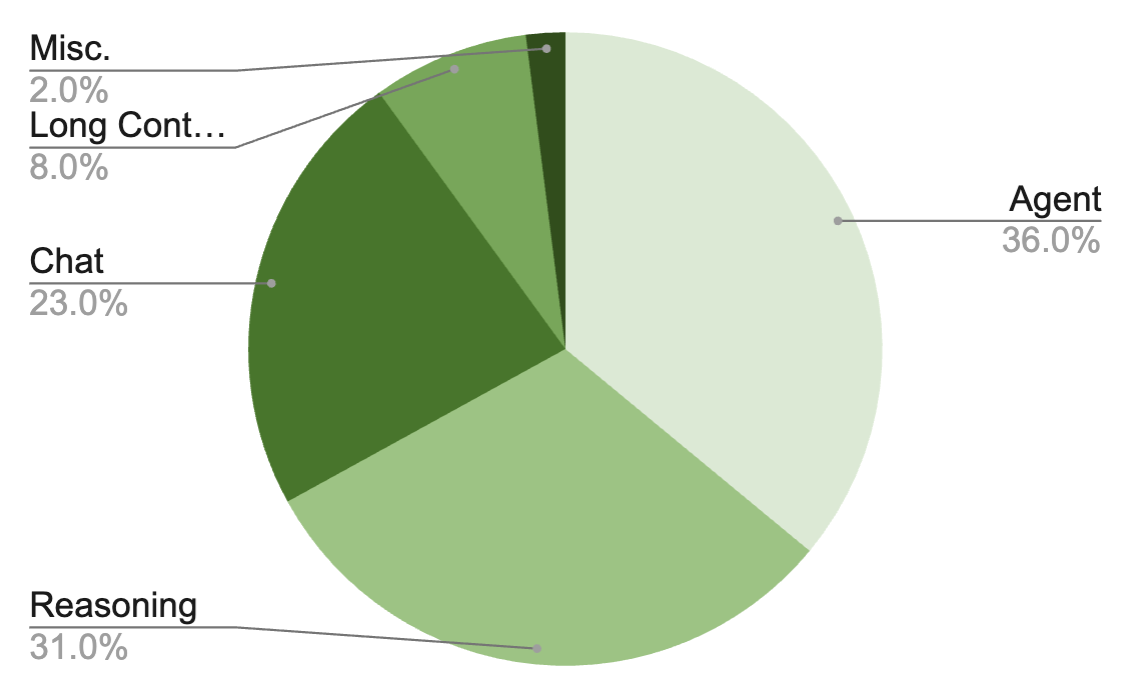
\includegraphics[width=10cm]{figures/super_sft_blend.jpg}
    \caption{SFT data blend for \ourmodel. }
    \label{fig:sft_blend}
\end{figure}


\subsubsection{Reasoning Control}

\ourmodel is trained for three reasoning modes: reasoning-off, regular and low-effort. The low-effort reasoning mode is a new addition.
The regular and low-effort reasoning modes have the option to be used in conjunction with inference-time budget control \citep{nvidia2025nemotronhfamilyaccurateefficient}.
These combinations of controls provide flexibilities that cover the entire spectrum of accuracy-efficiency trade-off to meet customers' needs in various application scenarios.

The low-effort reasoning mode is introduced during the SFT stage by adding training samples generated by GPT-OSS-120B in its low-effort mode \citep{du2025nemotron}.
These low-effort training samples cover the tasks of math reasoning, STEM question answering and instruction following, and represent 2\% of the overall SFT data by sample count.
The low-effort mode is later optimized during the RL stages to be discussed in the next section.

The SFT recipe for reasoning-off mode and for inference-time budget control is similar to \cite{nvidia2025nemotron3nanoopen} with a few differences.
We strip the reasoning traces from a random 3\% samples for reasoning-off mode.
After the main SFT stage, we add a short semi-on-policy SFT stage of 350 steps for inference-time budget control, where we collect roll-outs from the model and truncate 12\% of reasoning traces to random reasoning budgets.

%\ourmodel allows for three different forms of reasoning control: reasoning on/off control, token budget control, and a new reasoning low mode. To enable reasoning on/off control and budget control, we follow the same approach as \citep{nvidia2025nemotron3nanoopen}. To enable a reasoning low mode, we add low reasoning budget traces from GPT-OSS in the SFT stage, and conduct RL training to further improve the reasoning low mode performance.

